\chapter{Asociaciones entre clases}


Se representa mediante una línea continua entre las clases asociadas.
En este caso podemos saber que dado un libro podemos saber sus autores o viceversa.
Las asociaciones entre clases contienen 3 factores (cardinalidad, navegabilidad y multiplicidad).
\begin{itemize}
	\item La \textbf{cardinalidad} es el número de clases asociadas, por defecto, son binarias (cardinalidad = 2).
	\item La \textbf{multiplicidad} indica cuántos objetos de las clases se enlazan, en este caso como mínimo se enlaza 1 y como máximo muchos (1..*). Si no se especifica es 1.
	\item La \textbf{navegabilidad} indica el sentido de la relación, por defecto, son bidireccionales pero pueden existir asociaciones de \textit{A → B} o \textit{A ← B} (unidireccionales, donde el extremo de la flecha es el sentido).
\end{itemize}
Estas asociaciones pueden tener algunas dependencias (agregaciones y composiciones).
\section{Implementaciones}
Dependiendo de la multiplicidad que haya en cada extremo de las clases de objetos implemetaremos de una manera u 
otra las relaciones entre las clases.

Donde las relaciones que tienen una multiplicidad muchos - muchos se harán uso de tipos contendores asociativos o si la 
multiplicidad es 1 - 1 solamente se almacenará el objeto con el que se enlazan.

\subsection{Plantilla Implementación 1-N}
\begin{center}
\begin{lstlisting}[frame=single]
  class B; //declaracion adelantada
  class A{ //clase con multiplicidad 1
  public:
    //...
    typedef std::set<B*>Bs;
    void setB(B& b){bs_.insert(&b);}; //guardamos los elementos en el conjunto
    const Bs& getA() const{return bs_;}; //objeto B enlazado con A
  private:
    Bs bs_; //enlace con objeto B
  };
  class B{ //clase con multiplicidad N
  public:
    //...
    void setA(A& a){a_ = a;}
    const A& getB()const{return a_;}
  private:
    A a_;
  };
\end{lstlisting}
\end{center}
\newpage
\subsection{Implementación 1-1}

\begin{figure}[h]
    \centering
	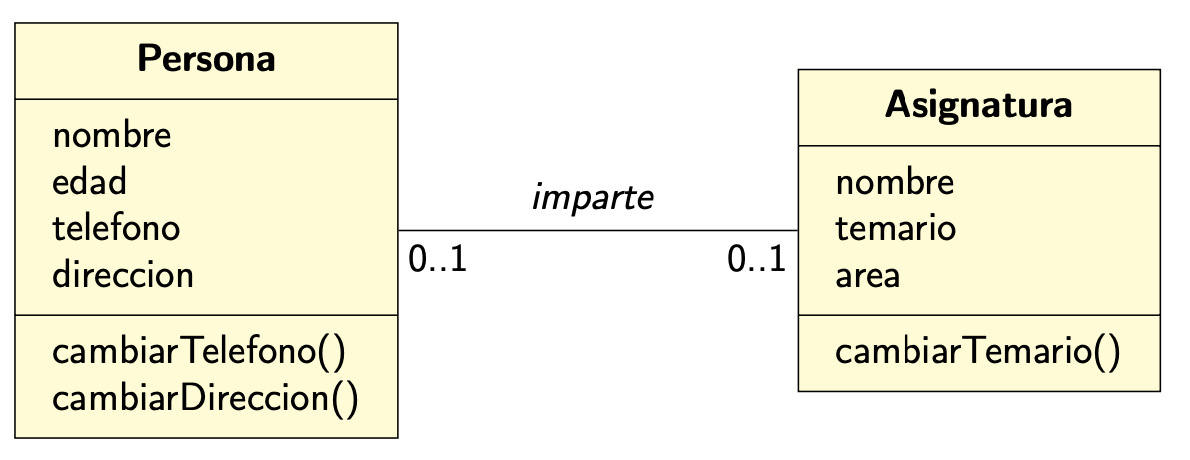
\includegraphics[width=\textwidth]{Imagenes/asociacion1.png}
    \caption{Asociación 1-1}
\end{figure}
\begin{center}
	\begin{lstlisting}[frame=single]
class Asignatura; //declaracion adelantada
class Persona{
  public:
  //...
  void setA(Asignatura& a){asig_ = &a;}; //enlazamos   
  //objeto Asignatura enlazado con Persona
  const Asignatura& getA() const noexcept {return *asig_;} 
  private:
  Asignatura* asig_; //enlace con objeto Asignatura
};
class Asignatura{
  public:
  //...
  void setP(Persona& p)noexcept{persona_ = &p;} //enlazamos
  const Persona& getP()const noexcept{return *persona_;} //objeto Persona enlazado con Asignatura
  private:
  Persona* persona_; //enlace con objeto Persona
};
\end{lstlisting}
\end{center}


\newpage
\subsection{Implementación N-M}
\begin{figure}[h]
    \centering
    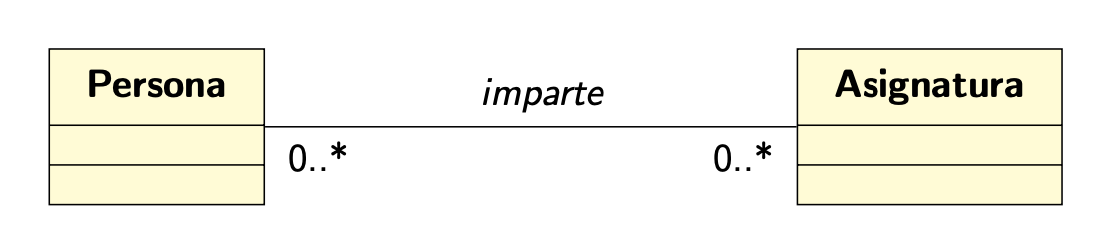
\includegraphics[width=\textwidth]{Imagenes/asociacion2.png}
    \caption{Asociación muchos - muchos}
\end{figure}

\begin{center}
	\begin{lstlisting}[frame=single]
class Asignatura;
class Persona{
  public:
    //...
    typedef set<Asignatura*> As;
    void setB(Asignatura& a)noexcept{as_.insert(&a);}
    const As& getA()const noexcept{return as_;}
  private:
    As as_;   
};

class Asignatura{
  public:
    //...
    typedef set<Persona*> Ps;
    void setP(Persona& p)noexcept{ps_.insert(&p);}
    const Ps& getB()const noexcept{return ps_;}
  private:
    Ps ps_;
};
\end{lstlisting}
\end{center}

